
\section{QSL-Karten}
\label{section:qsl_karten}
\begin{frame}%STARTCONTENT

\begin{columns}
    \begin{column}{0.48\textwidth}
    \begin{itemize}
  \item Nachweis darüber, dass eine Funkverbindung tatsächlich stattgefunden hat
  \item Dienen als Beleg bei der Beantragung von Amateurfunk-Diplomen
  \item Q-Gruppe QSL mit \enquote{ich bestätige den Empfang}
  \end{itemize}

    \end{column}
   \begin{column}{0.48\textwidth}
       
\begin{figure}
    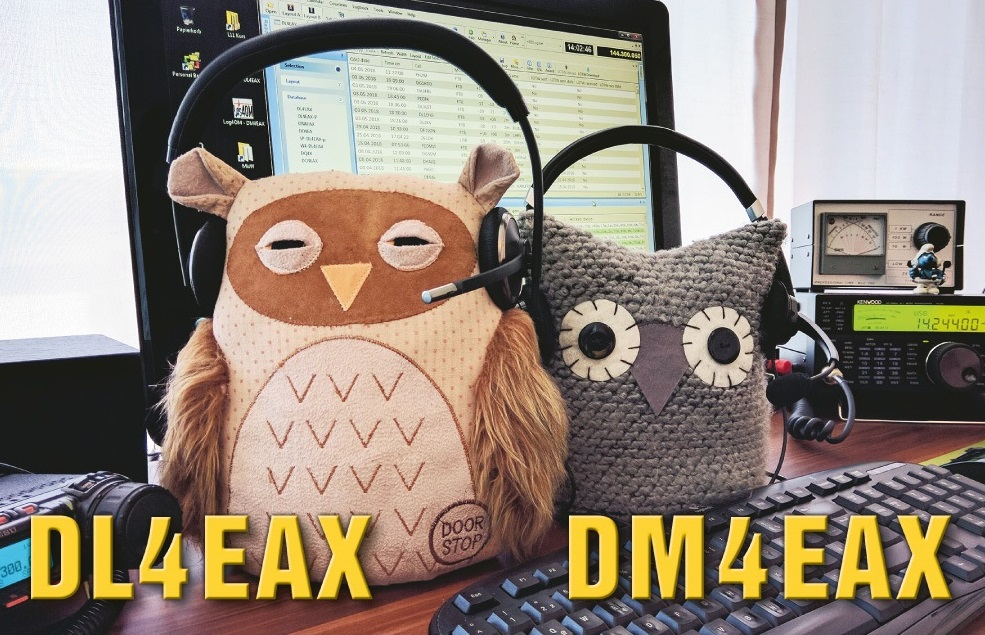
\includegraphics[width=0.85\textwidth]{foto/12}
    \caption{\scriptsize Gemeinsame QSL-Karte von DL4EAX und DM4EAX (Vorderseite)}
    \label{n_qsl_karten_vorderseite}
\end{figure}

   \end{column}
\end{columns}

\end{frame}

\begin{frame}
\only<1>{
\begin{QQuestion}{BG104}{Eine QSL-Karte ist~...}{eine Reservierungsbestätigung für die Teilnahme an einer Amateurfunkrunde. Sie sichert dem Funkamateur einen Listenplatz in der Runde.}
{die Bescheinigung über die Mitgliedschaft in einer Amateurfunkvereinigung.}
{eine Landkarte, in der Standorte für ortsgebundene Funkwettbewerbe eingezeichnet sind.}
{die Bestätigung einer Amateurfunkverbindung. Sie dient z. B. als Beleg bei der Beantragung von Amateurfunk-Diplomen.}
\end{QQuestion}

}
\only<2>{
\begin{QQuestion}{BG104}{Eine QSL-Karte ist~...}{eine Reservierungsbestätigung für die Teilnahme an einer Amateurfunkrunde. Sie sichert dem Funkamateur einen Listenplatz in der Runde.}
{die Bescheinigung über die Mitgliedschaft in einer Amateurfunkvereinigung.}
{eine Landkarte, in der Standorte für ortsgebundene Funkwettbewerbe eingezeichnet sind.}
{\textbf{\textcolor{DARCgreen}{die Bestätigung einer Amateurfunkverbindung. Sie dient z. B. als Beleg bei der Beantragung von Amateurfunk-Diplomen.}}}
\end{QQuestion}

}
\end{frame}

\begin{frame}
\frametitle{Angaben}

\begin{figure}
    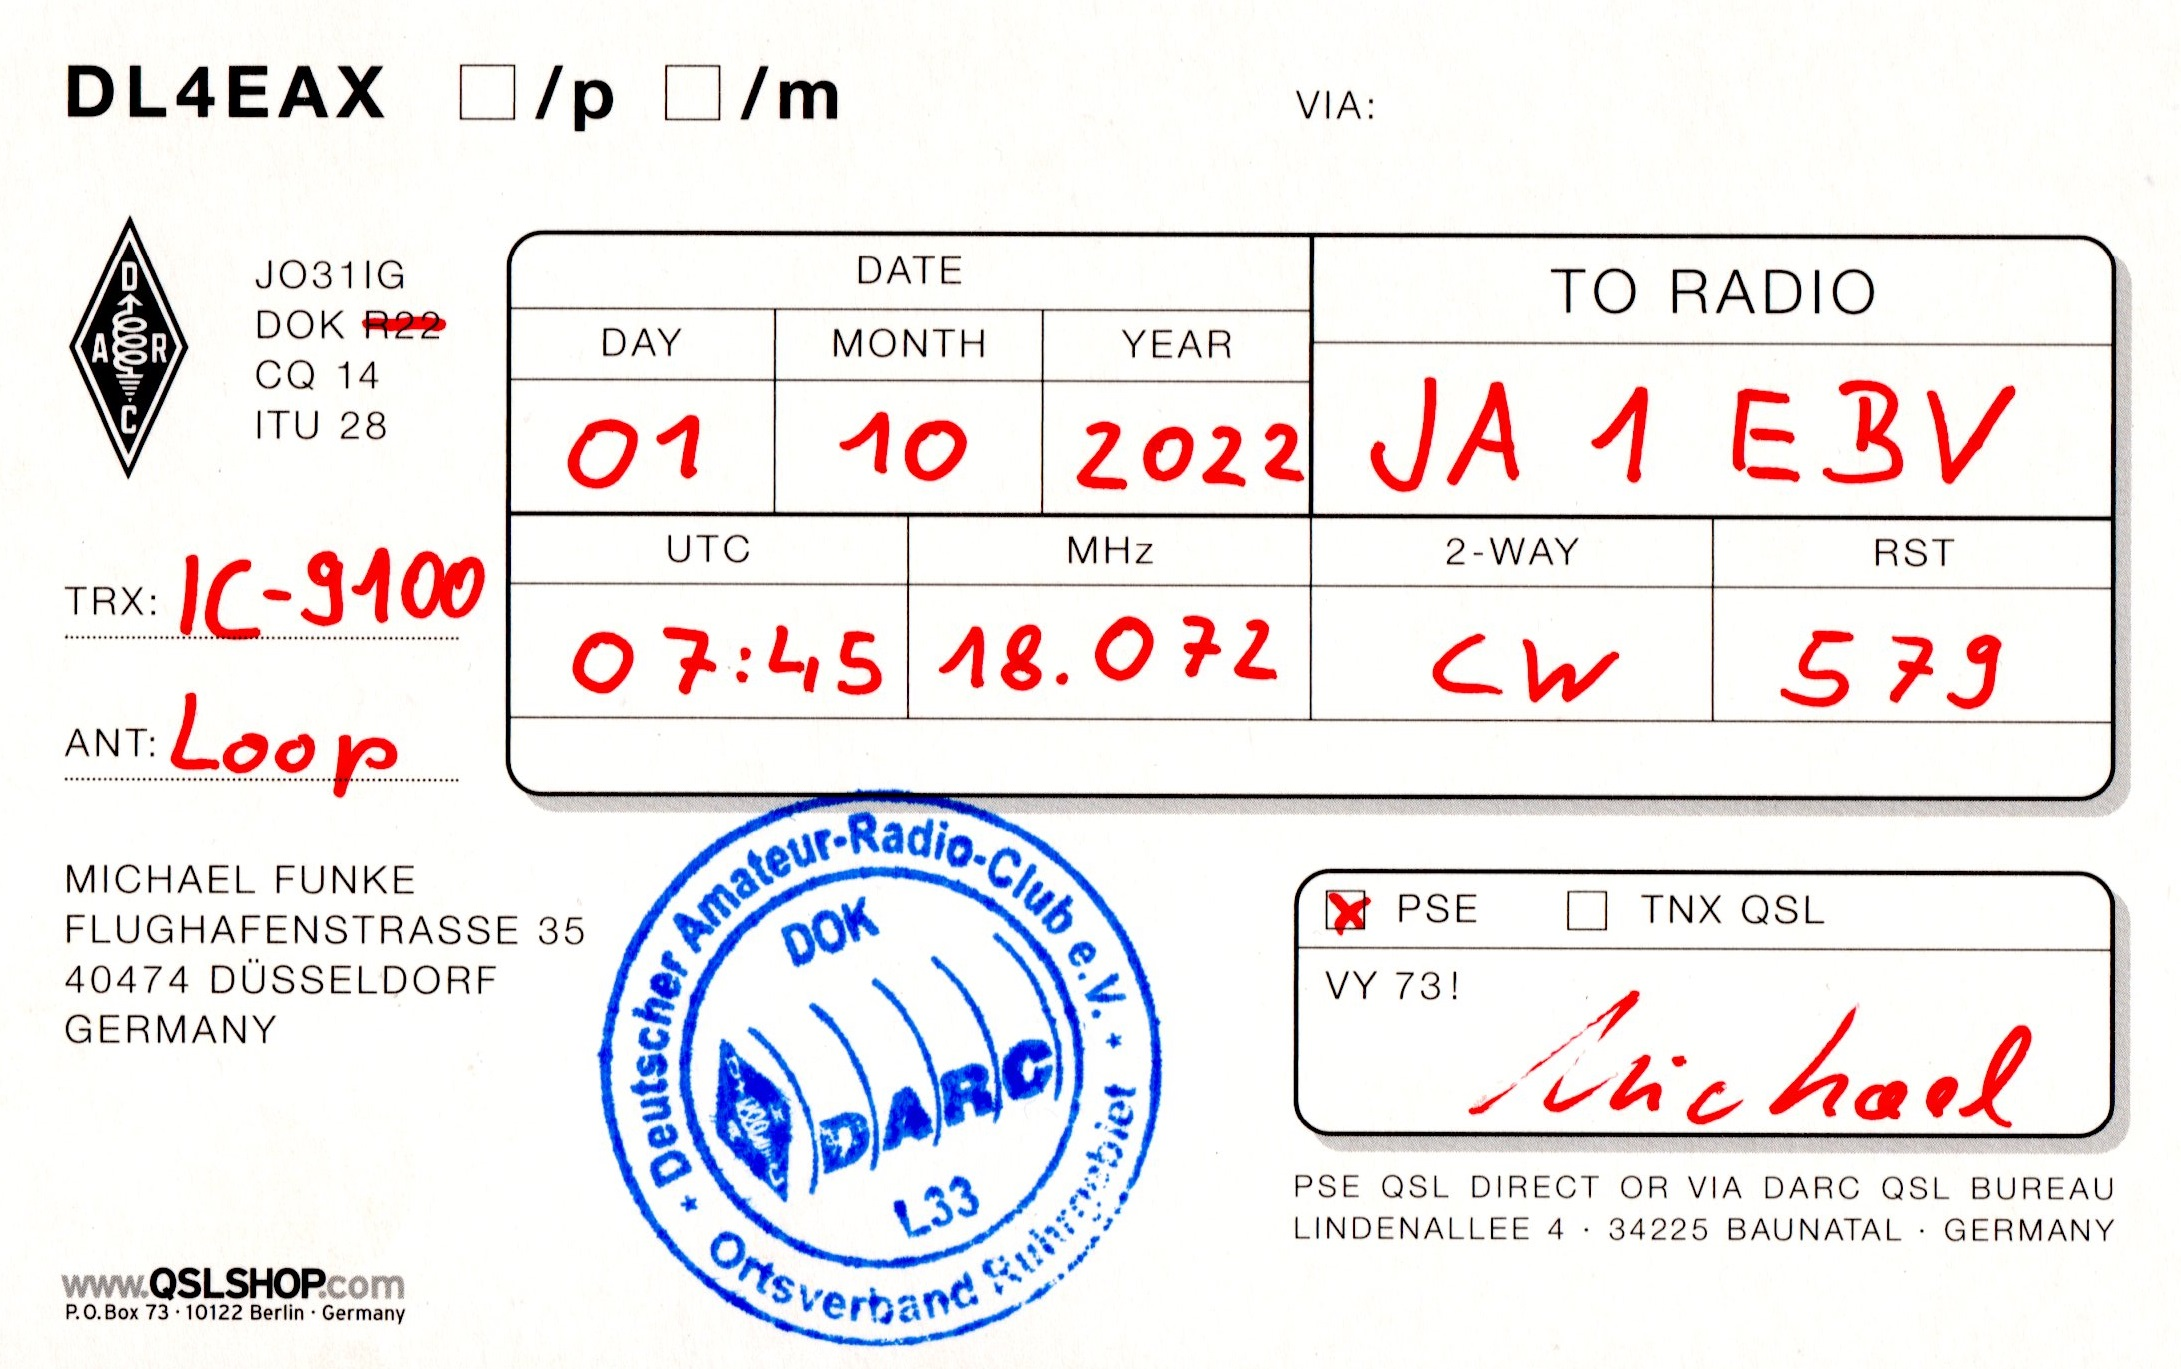
\includegraphics[width=0.85\textwidth]{foto/62}
    \caption{\scriptsize Beispiel für eine QSL-Karte, ausgestellt von DL4EAX zur Bestätigung einer Verbindung mit der Station JA1EBV}
    \label{n_qsl_karten_rueckseite_2}
\end{figure}
\end{frame}

\begin{frame}Eine QSL-Karte sollte mindestens folgende Angaben enthalten:

\begin{itemize}
  \item Datum
  \item Uhrzeit in UTC
  \item Eigenes Rufzeichen
  \item Rufzeichen der Gegenstation
  \item Genutzte Frequenz oder Frequenzband
  \item Verwendetes Übertragungsverfahren
  \item Gegebener Rapport
  \end{itemize}

\end{frame}

\begin{frame}
\only<1>{
\begin{QQuestion}{BG105}{Welche Angaben sollten QSL-Karten \underline{mindestens} enthalten?}{Verwendetes Rufzeichen, Datum und Uhrzeit der Funkverbindung in UTC, Frequenz, Übertragungsverfahren, Signal-Rapport sowie den eigenen Namen, Standort, Locator, die eigene Sendeleistung und Angaben zur eingesetzten technischen Ausrüstung}
{Verwendetes Rufzeichen, Rufzeichen der Gegenstation, Datum und Uhrzeit der Funkverbindung in UTC, Band, Übertragungsverfahren und Signal-Rapport}
{Rufzeichen der Gegenstation, Datum und Uhrzeit der Funkverbindung in UTC, genaue Frequenz, Übertragungsverfahren, Signal-Rapport und weitere übliche Angaben wie den eigenen Namen, Standort, Locator und die eigene Sendeleistung}
{Rufzeichen der Gegenstation, Datum und Uhrzeit der Funkverbindung in UTC, Frequenz, Übertragungsverfahren, Angaben über das Funkwetter und die Unterschrift des Operators}
\end{QQuestion}

}
\only<2>{
\begin{QQuestion}{BG105}{Welche Angaben sollten QSL-Karten \underline{mindestens} enthalten?}{Verwendetes Rufzeichen, Datum und Uhrzeit der Funkverbindung in UTC, Frequenz, Übertragungsverfahren, Signal-Rapport sowie den eigenen Namen, Standort, Locator, die eigene Sendeleistung und Angaben zur eingesetzten technischen Ausrüstung}
{\textbf{\textcolor{DARCgreen}{Verwendetes Rufzeichen, Rufzeichen der Gegenstation, Datum und Uhrzeit der Funkverbindung in UTC, Band, Übertragungsverfahren und Signal-Rapport}}}
{Rufzeichen der Gegenstation, Datum und Uhrzeit der Funkverbindung in UTC, genaue Frequenz, Übertragungsverfahren, Signal-Rapport und weitere übliche Angaben wie den eigenen Namen, Standort, Locator und die eigene Sendeleistung}
{Rufzeichen der Gegenstation, Datum und Uhrzeit der Funkverbindung in UTC, Frequenz, Übertragungsverfahren, Angaben über das Funkwetter und die Unterschrift des Operators}
\end{QQuestion}

}
\end{frame}

\begin{frame}
\only<1>{
\begin{QQuestion}{BG106}{Was sollten Sie bei der Eintragung von Uhrzeiten in QSL-Karten beachten? Sie sollten in~...}{der Ortszeit des Funkpartners eingetragen werden, damit es zu keinen Verwechselungen kommt.}
{der eigenen Ortszeit eingetragen werden, um den deutschen Vorschriften zu genügen.}
{der koordinierten Weltzeit (UTC) eingetragen werden, um Funkpartnern im Ausland das Auffinden im Logbuch zu erleichtern.}
{der eigenen Ortszeit und zusätzlich in der Ortszeit des Funkpartners eingetragen werden, um sowohl den deutschen Vorschriften zu genügen als auch Funkpartnern im Ausland das Auffinden im Logbuch zu erleichtern.}
\end{QQuestion}

}
\only<2>{
\begin{QQuestion}{BG106}{Was sollten Sie bei der Eintragung von Uhrzeiten in QSL-Karten beachten? Sie sollten in~...}{der Ortszeit des Funkpartners eingetragen werden, damit es zu keinen Verwechselungen kommt.}
{der eigenen Ortszeit eingetragen werden, um den deutschen Vorschriften zu genügen.}
{\textbf{\textcolor{DARCgreen}{der koordinierten Weltzeit (UTC) eingetragen werden, um Funkpartnern im Ausland das Auffinden im Logbuch zu erleichtern.}}}
{der eigenen Ortszeit und zusätzlich in der Ortszeit des Funkpartners eingetragen werden, um sowohl den deutschen Vorschriften zu genügen als auch Funkpartnern im Ausland das Auffinden im Logbuch zu erleichtern.}
\end{QQuestion}

}
\end{frame}

\begin{frame}
\only<1>{
\begin{QQuestion}{BG107}{Welche Uhrzeit tragen Sie in die QSL-Karte ein, wenn Sie um 15:30 MEZ ein QSO hatten?}{14:30 UTC}
{13:30 UTC}
{17:30 UTC}
{16:30 UTC}
\end{QQuestion}

}
\only<2>{
\begin{QQuestion}{BG107}{Welche Uhrzeit tragen Sie in die QSL-Karte ein, wenn Sie um 15:30 MEZ ein QSO hatten?}{\textbf{\textcolor{DARCgreen}{14:30 UTC}}}
{13:30 UTC}
{17:30 UTC}
{16:30 UTC}
\end{QQuestion}

}
\end{frame}

\begin{frame}
\only<1>{
\begin{QQuestion}{BG108}{Welche Uhrzeit tragen Sie in die QSL-Karte ein, wenn Sie um 13:30 MESZ eine Funkverbindung hatten?}{11:30 UTC}
{13:30 UTC}
{12:30 UTC}
{14:30 UTC}
\end{QQuestion}

}
\only<2>{
\begin{QQuestion}{BG108}{Welche Uhrzeit tragen Sie in die QSL-Karte ein, wenn Sie um 13:30 MESZ eine Funkverbindung hatten?}{\textbf{\textcolor{DARCgreen}{11:30 UTC}}}
{13:30 UTC}
{12:30 UTC}
{14:30 UTC}
\end{QQuestion}

}
\end{frame}

\begin{frame}
\frametitle{Vermittlung von QSL-Karten}
\begin{itemize}
  \item Über teilnehmende Amateurfunkverbände in den Ländern
  \item via Vermittlungsbüro -- international \enquote{Bureau}
  \item Weltweites alternatives Postnetz
  \item In Deutschland bietet das der DARC e.V. für Mitglieder kostenlos an
  \end{itemize}

\end{frame}

\begin{frame}
\frametitle{Callbooks}
\begin{itemize}
  \item Adressen in internationalen Amateurfunk-Rufzeichenlisten (Callbook)
  \item Oder im Internet
  \item Es gibt \enquote{QSL-Manager}, die für andere Stationen den Versand übernehmen
  \end{itemize}

\end{frame}

\begin{frame}
\only<1>{
\begin{QQuestion}{BG110}{Wo können Sie die Anschriften von ausländischen Funkamateuren finden, denen Sie die QSL-Karte direkt zusenden möchten?}{Ich finde diese in der VO Funk.}
{Ich finde diese in der Amateurfunk-Rufzeichenliste auf den Internetseiten der Bundesnetzagentur.}
{Ich finde diese in der internationalen Amateurfunk-Rufzeichenliste (Callbook) oder aus Informationen des Internets.}
{Ich finde diese im internationalen Telefonbuch.}
\end{QQuestion}

}
\only<2>{
\begin{QQuestion}{BG110}{Wo können Sie die Anschriften von ausländischen Funkamateuren finden, denen Sie die QSL-Karte direkt zusenden möchten?}{Ich finde diese in der VO Funk.}
{Ich finde diese in der Amateurfunk-Rufzeichenliste auf den Internetseiten der Bundesnetzagentur.}
{\textbf{\textcolor{DARCgreen}{Ich finde diese in der internationalen Amateurfunk-Rufzeichenliste (Callbook) oder aus Informationen des Internets.}}}
{Ich finde diese im internationalen Telefonbuch.}
\end{QQuestion}

}
\end{frame}

\begin{frame}
\only<1>{
\begin{QQuestion}{BG109}{HZ1HZ sagte Ihnen \glqq QSL via K8PYD\grqq{}. Was würden Sie tun, um die QSL-Karte von HZ1HZ zu erhalten?}{Ich warte, bis HZ1HZ die Karte an K8PYD geschickt hat.}
{Ich muss meine QSL-Karte via HZ1HZ senden, weil K8PYD der QSO-Partner war.}
{Ich schaue im Callbook nach der Adresse von HZ1HZ und schicke die Karte direkt.}
{Ich sende meine QSL-Karte via K8PYD, weil dieser der QSL-Manager von HZ1HZ ist.}
\end{QQuestion}

}
\only<2>{
\begin{QQuestion}{BG109}{HZ1HZ sagte Ihnen \glqq QSL via K8PYD\grqq{}. Was würden Sie tun, um die QSL-Karte von HZ1HZ zu erhalten?}{Ich warte, bis HZ1HZ die Karte an K8PYD geschickt hat.}
{Ich muss meine QSL-Karte via HZ1HZ senden, weil K8PYD der QSO-Partner war.}
{Ich schaue im Callbook nach der Adresse von HZ1HZ und schicke die Karte direkt.}
{\textbf{\textcolor{DARCgreen}{Ich sende meine QSL-Karte via K8PYD, weil dieser der QSL-Manager von HZ1HZ ist.}}}
\end{QQuestion}

}
\end{frame}

\begin{frame}
\frametitle{Elektronische QSL-Karten}
\begin{itemize}
  \item Papierlose Alternativen
  \item Elektronische Logbücher lassen sich hochladen
  \item Nur wenige Plattformen werden für Diplome anerkannt
  \end{itemize}
\end{frame}

\begin{frame}
\only<1>{
\begin{QQuestion}{BG111}{Welche Alternativen zur QSL-Karte sind üblich? Bestätigung von Funkverbindungen durch~...}{elektronische QSL-Karten oder Logbuch-Upload}
{die BNetzA als unabhängige Stelle}
{das Intruder Monitoring der Amateurfunkverbände}
{Beurkundung durch einen Notar oder SWL-Fachanwalt}
\end{QQuestion}

}
\only<2>{
\begin{QQuestion}{BG111}{Welche Alternativen zur QSL-Karte sind üblich? Bestätigung von Funkverbindungen durch~...}{\textbf{\textcolor{DARCgreen}{elektronische QSL-Karten oder Logbuch-Upload}}}
{die BNetzA als unabhängige Stelle}
{das Intruder Monitoring der Amateurfunkverbände}
{Beurkundung durch einen Notar oder SWL-Fachanwalt}
\end{QQuestion}

}
\end{frame}%ENDCONTENT
